\newpage

\subsection{Administración de datos} \label{seccionAdmDatos}

% gráficos de ADM de datos (las tres páginas seguidas, y luego la explicación).
\begin{figure}[H]
   \centering
   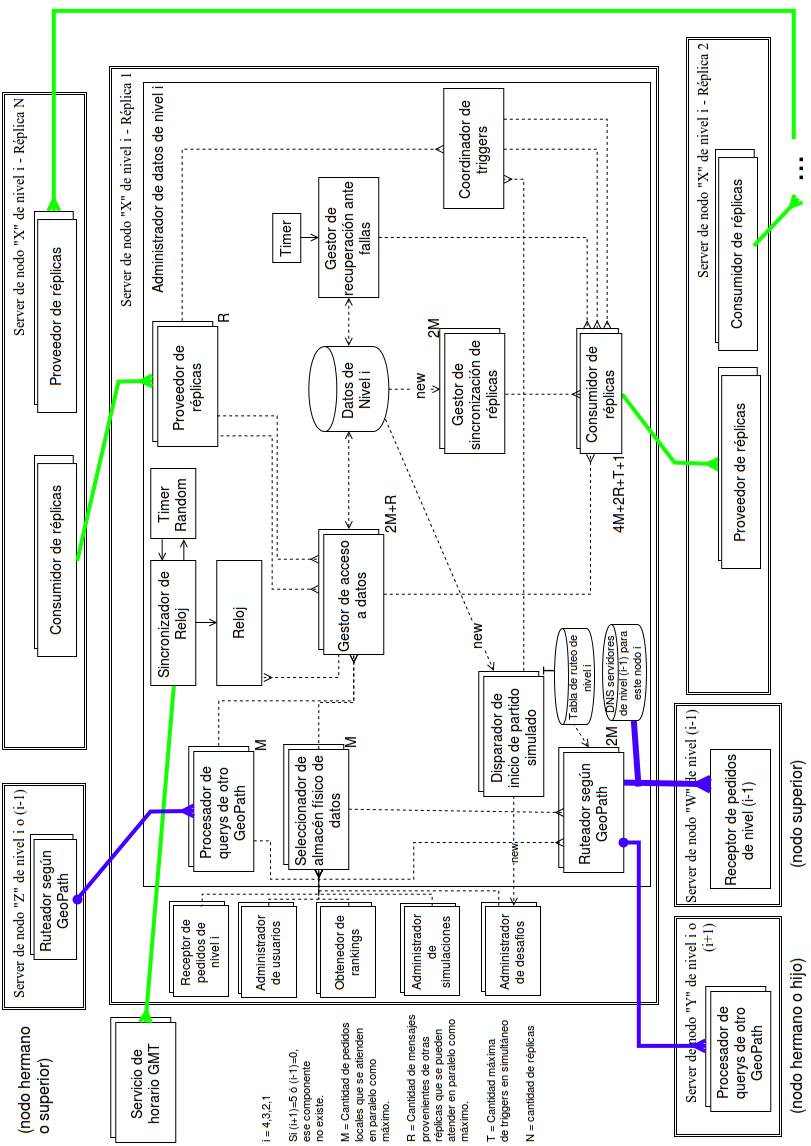
\includegraphics[height=0.93\textheight]{reentrega/imagenes/admDatos.png}
   \caption{Componente administrador de datos de nivel i.}
\end{figure}

\begin{figure}[H]
   \centering
   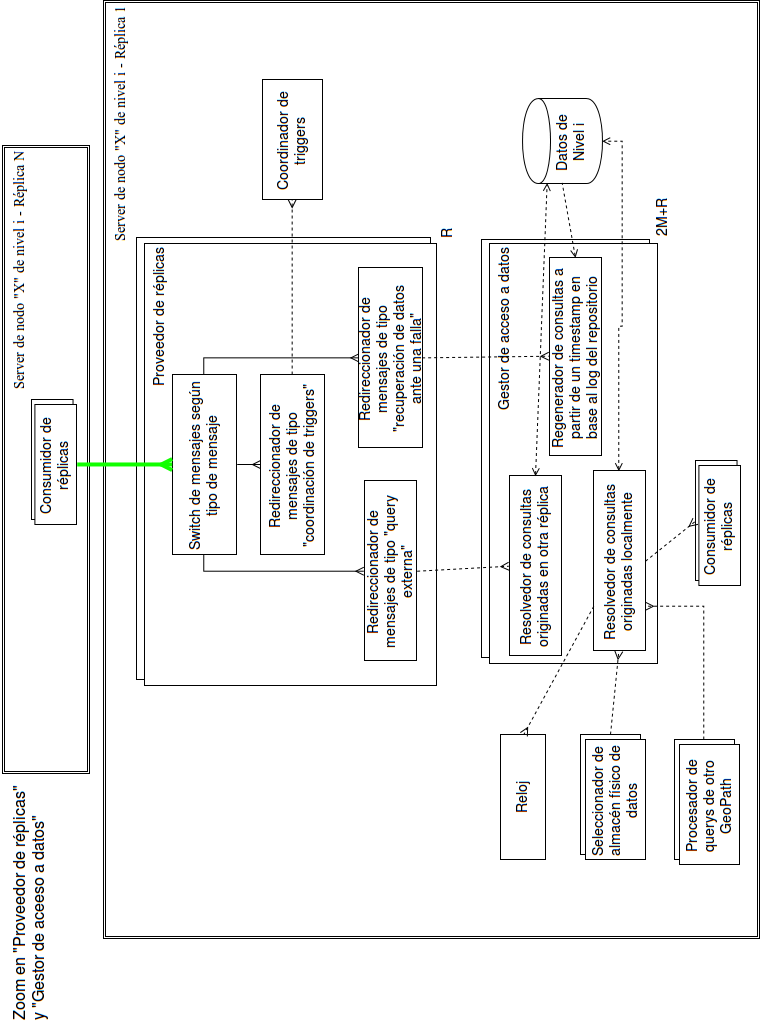
\includegraphics[height=0.93\textheight]{reentrega/imagenes/admDatos-zoom1.png}
   \caption{Zoom en ``Proveedor de réplicas'' y ``Gestor de acceso a datos''.}
\end{figure}

\begin{figure}[H]
   \centering
   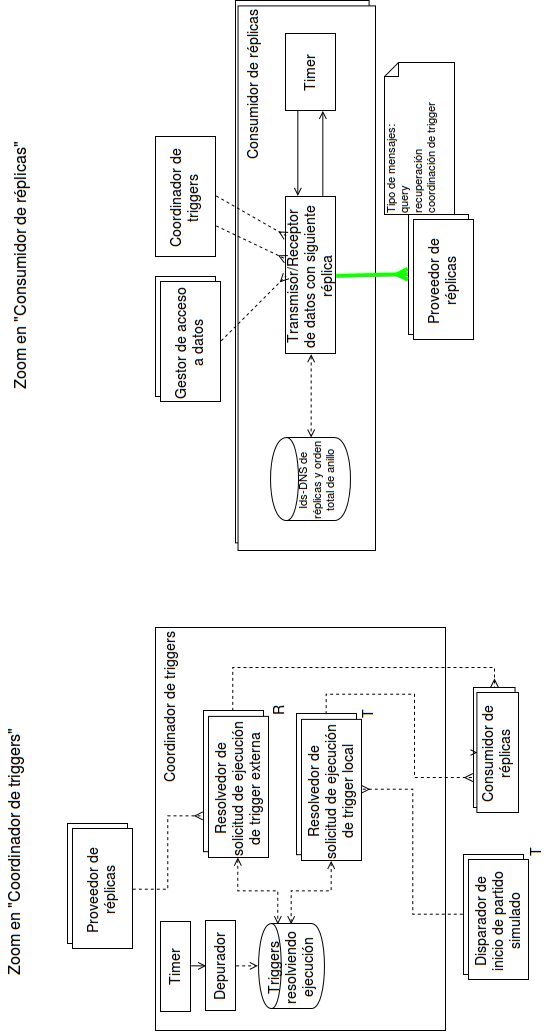
\includegraphics[height=0.93\textheight]{reentrega/imagenes/admDatos-zoom2.png}
   \caption{Zoom en ``Proveedor de réplicas'' y ``Coordinador de triggers''.}
\end{figure}

En cada nodo de nivel i (Ej: CABA en nivel 4) hay uno o más servidores. Cada uno tiene un servidor HTTP  y un Data Server con los datos de ese nodo. Todos los servidores en un mismo nodo son réplicas tanto de software como de datos. Por ejemplo, para el GeoPath $<$Sudamérica, Argentina, Bs.As., CABA$>$ tenemos 10 servidores de nivel 4, donde cada uno tiene el mismo software y los mismos datos.

Los relojes de todos los servidores de nivel i están sincronizados.
Dentro del componente ``Administrador de Datos'' hay un ``Sincronizador de Reloj'' que se ejecuta cada cierta cantidad de minutos entre 1 y 5, definida aleatoriamente cada vez. Este componente accede a un servicio online que provee la hora GMT. Los minutos se eligen aleatoriamente para evitar que todos los servidores accedan al mismo tiempo al servicio web y lo saturen. El proveedor del servicio nos confirmó que usando esta  estrategia el servicio respondería siempre. Además nos aseguró que tiene una réplica de su servicio hosteada en cada país, para reducir el tiempo de respuesta. De esta manera, todos los servidores de nivel i se encuentran sincronizados al horario GMT.

Cada registro en los repositorios de datos tiene asociado un timestamp correspondiente a la última actualización.

\subsubsection{Replicación de datos y manejo de fallas}

Cada servidor escribe y lee los datos de su réplica local, salvo que ésta no responda. Supongamos primero que la réplica local funciona correctamente. Luego de realizar una escritura, el “Seleccionador de almacén físico de datos” envía la query al “Gestor de Acceso a Datos” por determinado puerto, que le indica al gestor que la query se originó localmente. Luego le asigna un timestamp (TS) a la query y la ejecuta en el repositorio local. Si la query produjo un cambio en los datos, se dispara automáticamente el proceso “Gestor de sincronización de réplicas” (con un trigger) al que se le asigna como input la metadata de los cambios producidos en los datos locales. Este genera una query para actualizar y sincronizar las demás réplicas, la cual incluye el timestamp generado previamente (TS).

La estructura de réplicas tiene forma de anillo, donde cada par de réplicas se comunica utilizando “Consumidor de réplicas” y “Proveedor de réplicas”, mediante un conector seguro (SSL). Entonces el “Gestor de sincronización de réplicas” envía la query con el TS al “Consumidor de réplicas” y este a su vez envía la query al “Proveedor de réplicas” del siguiente servidor en el anillo.

El “Proveedor de réplicas” luego envía la query al “Gestor de acceso a datos” por un puerto especial, que le indica que la query es externa, entonces antes de impactarla, verifica los datos que serán alterados y compara el TS con el TS de cada registro. De esta manera detecta si localmente hay una actualización posterior a la que llegó de afuera (o si ya tiene la misma), y en tal caso la descarta y no la impacta. Este mecanismo no sólo prioriza la escritura más reciente para evitar condiciones de carrera sino que además permite cortar el ciclo de actualizaciones (cuando llega nuevamente a la réplica que originó la actualización, el TS de la query y del registro será el mismo y no se impactará).

Cabe aclarar que si una query externa fue descartada porque la copia local contenía un dato más nuevo, este dato ya fue enviado hacia las siguientes réplicas del anillo, por ende no tiene sentido propagar la query externa que quedó vieja.

Ahora veremos el caso en el que la réplica local de datos falla y debemos utilizar una réplica externa. En tal caso, el “Gestor de acceso a datos” detectará con un timeout que hubo un problema en la copia local y encenderá internamente un flag indicando que la copia local no se puede usar. Además seteará un timer para que en 10 minutos se apague el flag y se pueda reintentar con la copia local.

Dado que la query se generó en este servidor, aunque no haya podido impactarse, le agrega un timestamp y luego la envía al “Consumidor de réplicas”, que la transmite y la impacta usando el “Proveedor de réplicas” de la misma manera que antes.

Si llega una query al “Proveedor de réplicas” mientras la réplica local está inutilizable, el componente la envia al “Gestor de acceso a datos”, el cual la redirige al “Consumidor de réplicas” sin siquiera intentar utilizar el repositorio local (hasta que se apague automáticamente el flag).

Todo el mecanismo descripto se basa en la estrategia transaccional utilizada por Cassandra. Localmente en cada repositorio utiliza transacciones ACID (que garantizan principalmente la atomicidad y durabilidad de las escrituras) y a nivel global se garantiza consistencia eventual (asumimos que los datos terminan de propagarse por el anillo en a lo sumo 30 segundos). Esto permite tener las réplicas eventualmente consistentes, garantizando alta disponibilidad (si una réplica falla) y performance (no es necesario escribir en todas las réplicas y esperar ACKs por cada transacción). La única desventaja es que si se acceden a dos réplicas distintas en un intervalo muy corto de tiempo podrían verse datos distintos, pero como los servidores de nivel 5 tienen preferencia por uno de nivel 4 y siempre usan el mismo (salvo fallas), en general un mismo usuario accederá siempre al mismo servidor de nivel 4 y verá los mismos datos. Si un usuario crea un desafío, quizás sus amigos tengan que refrescar el sitio varias veces para ver el nuevo desafío en la lista.

\subsubsection{Triggers programados por reloj}

Los partidos de los desafíos registrados en un nodo de nivel i son ejecutados en el mismo nodo (simulados o liga de fantasía). Pero cada partido podría ejecutarse en cualquiera de las réplicas dentro del nodo. Físicamente, el trigger que dispara el inicio de un partido a determinada hora se registra en todas las réplicas. Dado que comparten el reloj, deberían disparar el trigger todas al mismo tiempo aproximadamente. Una vez que el trigger es disparado, lo recibe el “Disparador de inicio de partido simulado”, que antes de enviarlo al “Administrador de Desafíos”, le envía una consulta a un “Coordinador de Triggers”, indicando todos los metadatos necesarios para identificar el trigger disparado por el repositorio.

Dentro del “Coordinador de Triggers”, la solicitud es procesada por “Resolvedor de solicitud de ejecución de trigger local” que almacena en un repositorio interno los metadatos del trigger (IdTrigger) y luego genera un número aleatorio entre 0 y 1 (Rnd). Si el IdTrigger ya se encontraba en el repositorio, debería haber un flag indicando que no será ejecutado localmente, y el proceso termina (ver más adelante por qué puede suceder esto). Finalmente, envía un mensaje al “Coordinador de Triggers” que está siguiente en el anillo (mediante el “Consumidor de réplicas”), indicando los siguientes datos:

\begin{itemize}
	\item IdTrigger
	\item Id de la réplica donde se originó el trigger (ej: 1)
	\item Número aleatorio más grande encontrado para la ejecución de este trigger (Rnd)
	\item Id de la réplica que tiene el número aleatorio más grande
\end{itemize}

Este paquete debe dar toda la vuelta en el anillo. A medida que vaya pasando por cada “Coordinador de Triggers” del anillo, estos observarán el número aleatorio que generaron localmente y si es más grande, cambiarán los últimos dos campos (en breve explicaremos cómo). Luego de dar toda la vuelta, el paquete llega al “Coordinador de triggers” de la réplica original, que detectará que es la original por el segundo campo, y luego observa el último campo, que indica quién ejecutará el trigger. De esta manera, la réplica que haya obtenido el número aleatorio más alto ejecutará el trigger.

Dentro del “Coordinador de Triggers” se encuentra el “Resolvedor de solicitud de ejecución de trigger externa”, que recibirá paquetes como el descripto previamente, proveniente de la réplica anterior en el anillo. Este componente tomará cada paquete e inspeccionará primero el segundo campo:

\begin{enumerate}
	\item Si el paquete se originó en la réplica actual, quiere decir que ya dio toda la vuelta al anillo y el cuarto campo indica qué réplica debe ejecutar el trigger. Entonces en el repositorio de “Triggers resolviendo ejecución” se marca con un flag si debe ejecutarse localmente o no. Luego el “Resolvedor de solicitud de ejecución de trigger local” que había tomado la solicitud inicial observará el cambio en el repositorio y responderá a quién lo solicitó.

	\item Si el paquete se originó en otra réplica, compara el número aleatorio con el número aleatorio local (que lo lee de “Triggers resolviendo ejecución”). Si es más grande el local, se actualiza el paquete y se envía al siguiente en el anillo. Si casualmente el número aleatorio es igual (un caso muy poco probable), se utiliza el id de réplica para desempatar (gana la más grande).

\begin{enumerate}
		\item Si por alguna razón el IdTrigger no se encuentra en “Triggers resolviendo ejecución”, se agrega el IdTrigger al repositorio y se marca con el flag de que no será ejecutado localmente, y el paquete se pasa al siguiente en el anillo tal cual se recibió. De esta manera si el trigger es disparado más tarde localmente, directamente se desestima ya que fue ejecutado en otra réplica.
\end{enumerate}
\end{enumerate}


De esta manera hay una única réplica que ejecuta la simulación de un partido, ya que sólo un “Administrador de datos” enviará el disparador hacia el “Administrador de desafíos”. La ejecución de un trigger se podrá demorar a lo sumo 30 segundos (el tiempo máximo en dar una vuelta al anillo).

Cada 24hs se ejecuta un “Depurador” que borra las entradas de “Triggers resolviendo ejecución” que ya están resueltas (flag de ejecución o no ejecución encendido) hace más de 24hs.


\subsubsection{Recuperación ante fallas}

Si un servidor del anillo falla en su totalidad (o falla la comunicación), el componente “Consumidor de réplicas” internamente setea un timer cada vez que envía un mensaje. Si el timer genera un aviso (timeout), componente “Transmisor/Receptor de datos con siguiente réplica” inspecciona su repositorio interno donde tiene la estructura del anillo y busca el siguiente integrante del anillo. Entonces se comunica directamente con el siguiente en el anillo.

Cuando un servidor vuelve a levantarse (o cuando el repositorio vuelve a funcionar), hay un proceso que está continuamente monitoreando el repositorio y descubre este evento (“Gestor de recuperación ante fallas”). Este proceso se encarga de verificar los logs del repositorio para ver el timestamp de la última transacción y envía un pedido de recuperación con ese timestamp al “Consumidor de réplicas”. Este mensaje llega a través del “Proveedor de réplicas” al “Gestor de acceso a datos” (por un canal especial). Luego el “Gestor de acceso a datos” busca todas las actualizaciones que hubo en su repositorio local desde el timestamp indicado hasta el momento y las retorna por el mismo canal. Estas actualizaciones llegan nuevamente al “Gestor de recuperación ante fallas”, que persiste los datos verificando los timestamps (por si ya hay datos nuevos en el repositorio recuperado). 


\subsubsection{Acceso a nodos de distinto GeoPath}

Esto lo detecta el “Seleccionador de almacén físico de datos”, que en caso de no corresponder el GeoPath al nodo actual, lo envía al “Ruteador según GeoPath”. Este componente utiliza una “Tabla de ruteo de nivel i”. Esta tabla permite rutear la solicitud a:

\begin{itemize}
	\item Un nodo hijo de este GeoPath, de nivel i+1 (Ej: de $<$Sudamérica,Argentina$>$ ir a $<$Sudamérica, Argentina, Bs.As., CABA$>$, pero no a $<$Europa, España, Barcelona, Barcelona$>$). Si i=4 esto no es posible ya que en nivel 5 no hay datos.
	\item Un nodo hermano de este GeoPath, de nivel i (Ej: de $<$Sudamérica,Argentina$>$ ir a $<$Sudamérica, Chile$>$, pero no se puede ir a $<$Europa, España$>$).
	\item El nodo superior de este GeoPath, de nivel i-1 (Ej: de $<$Sudamérica,Argentina$>$ ir a $<$Sudamérica$>$, pero no a $<$Europa$>$). Si i=1, no es posible esta navegación porque no hay nodo superior.
\end{itemize}

Este esquema permite que desde cualquier nodo se pueda escribir en cualquier otro usando el GeoPath correcto, pero la navegación se realiza a través del árbol sin saltear niveles. Esto reduce la cantidad de pedidos que puedan subir al nivel 1 desde muchos de nivel 4 y a la vez impide que haya muchos servidores de distintos niveles y regiones que escriban datos en un mismo nodo de nivel 4 (que contiene datos de usuarios y es posible que muchas veces sea necesario hacerlo).

Las tablas de ruteo tienen para cada GeoPath varios nombres de dominio de las distintas réplicas del nodo que cubre ese GeoPath.

Por ejemplo:
\begin{itemize}
	\item Tabla de ruteo de nivel 1 podría contener: (observar que no contiene entrada de nivel 1 porque no hay otro nodo de nivel 1, sólo hay réplicas).
	
	\begin{center}
	\begin{tabular}{| c | c |}
	\hline
	GeoPath & DNS \\
	\hline
	$<$Sudamérica$>$ & sudamerica.n2.s1.currygame.com, sudamerica.n2.s2.currygame.com\\
	\hline
	$<$África$>$ & africa.n2.s1.currygame.com\\
	\hline
	\end{tabular}
	\end{center}
	
	\item Tabla de ruteo de nivel 2 de Sudamérica podría contener:

	\begin{center}
	\begin{tabular}{| c | c |}
	\hline
	GeoPath & DNS \\
	\hline
	$<$Sudamérica,Argentina$>$ &  ar.n3.s1.currygame.com\\
	\hline
	$<$África$>$ & africa.n2.s1.currygame.com\\
	\hline
    $<$ $>$ &  n1.s1.currygame.com\\
	\hline
	\end{tabular}
	\end{center}
	
	\item Tabla de ruteo de nivel 3 de Argentina podría contener:
	\begin{center}
	\begin{tabular}{| c | c |}
	\hline
	GeoPath & DNS \\
	\hline
	$<$Sudamérica, Argentina, Bs.As., CABA$>$ & caba.ar.n4.s1.currygame.com\\
	\hline
	$<$Sudamérica,Argentina$>$ &  ar.n3.s1.currygame.com\\
	\hline
	$<$Sudamérica$>$ &  sudamerica.n2.s1.currygame.com\\
	\hline
	\end{tabular}
	\end{center}
	
	\item Tabla de ruteo de nivel 4 de CABA podría contener:
	\begin{center}
	\begin{tabular}{| c | c |}
	\hline
	GeoPath & DNS \\
	\hline
	$<$Sudamérica,Argentina$>$ &  ar.n3.s1.currygame.com\\
	\hline
	$<$Sudamérica, Argentina, Bs.As., Lanús$>$ & lanus.ar.n4.s1.currygame.com\\
	\hline
	\end{tabular}
	\end{center}

\end{itemize}


Las réplicas no están contenidas en la tabla de ruteo porque las réplicas se manejan desde el proveedor y consumidor de réplicas.

Si la query corresponde a una entrada del mismo nivel i o un nivel inferior (i+1), el ruteador enviará por un canal seguro la query a una de las réplicas de ese nodo (elegida al azar). Además este canal tiene una caché para acceder rápidamente a lecturas que ya fueron realizadas recientemente. La query es recibida por el “Procesador de Querys de otro GeoPath”, que si detecta que se puede resolver localmente, la envía al “Gestor de acceso a datos” por el mismo puerto que ingresan las querys locales y de esta manera se hace transparente la procedencia. Si no se puede resolver localmente porque corresponde a otro GeoPath, la envía a su ruteador para que este la redirija a donde corresponda.

Si la query corresponde a una entrada de un nivel superior (i-1) se envía al “Resolvedor de pedidos de nivel (i-1)” de cualquiera de las réplicas (elegida aleatoriamente), el cual procesará el pedido entrante y responderá de forma transparente. En este caso también hay caché y además se tiene un servidor favorito de nivel (i-1) y otras réplicas en caso de que el favorito no conteste. Si el favorito no contesta, en 10 minutos se reintenta utilizar y mientras se usan las réplicas elegidas aleatoriamente. Este esquema del favorito permite mantener la estructura de árbol incluso con las réplicas y así distribuir la carga.

Si la query corresponde a otro nivel o a un nodo que no es pariente, será descartada ya que no se permite ese acceso.

Por ejemplo, si a una de las réplicas del nodo de $<$Sudamérica$>$ llega el pedido de sumar fichas a un usuario de CABA que ganó un premio en un desafío sudamericano, el circuito es este:
\begin{enumerate}
	\item Desde $<$Sudamérica$>$ se redirige a $<$Sudamérica,Argentina$>$.
	\item Luego se redirige a $<$Sudamérica, Argentina, Bs.As., CABA$>$.
	\item Luego se resuelve localmente porque coincide el GeoPath local con el de la consulta.
\end{enumerate}

Si en cambio se desea inscribir un participante de CABA en un desafío Sudamericano, el GeoPath del desafío es $<$Sudamérica$>$ y el camio es:
\begin{enumerate}
	\item Desde $<$Sudamérica, Argentina, Bs.As., CABA$>$ se envía a $<$Sudamérica, Argentina$>$ en la réplica favorita si es posible, o en otra réplica random si no fuera posible.
	\item Luego como no coincide el GeoPath, se redirige a $<$Sudamérica$>$ siguiendo el mismo esquema de favoritismo.
	\item Luego se resuelve localmente y se almacena el participante con el equipo elegido.
\end{enumerate}


\subsubsection{Datos almacenados en nivel 4}

\begin{itemize}
	\item Usuarios registrados en el GeoPath asignado al nodo de nivel 4, ej: usuarios de $<$Sudamérica, Argentina, Bs.As., CABA$>$.
	\begin{itemize}
		\item Datos personales
		\item Datos de autenticación (la encripción de la contraseña se realiza por fuera).
		\item GeoPath (el mismo del servidor ya que no se registran usuarios de otro GeoPath)
		\item Tarjetas de Crédito (la encripción es responsabilidad del Administrador de usuarios)
		\item Fichas disponibles
		\item Desafíos en los que está inscripto (GeoPath de donde se creó el desafío, IdDesafio y puntaje).
		\item Puntos en el ranking de país.
		\item Equipos armados (ids de jugadores incluidos en cada equipo)
	\end{itemize}

	\item Desafíos creados por usuarios registrados en este GeoPath (en cualquier estado, incluso los que ya terminaron).
	\begin{itemize}
		\item GeoPath y IdUsuario de cada participante inscripto, junto con el equipo (con todos los ids de los jugadores que eligió en el equipo).
		\item Estado del desafío (abierto para inscripciones, jugando, terminado).
		\item Tabla de posiciones
		\item Logs de simulación (si es simulado).
		\item Fecha y hora de comienzo del desafío y de cada fecha/partido.
	\end{itemize}

	\item Jugadores reales disponibles para armar un equipo.
	
	\item Publicidad.
\end{itemize}


\subsubsection{Datos almacenados en nivel 3}

\begin{itemize}
	\item Usuarios administradores a nivel país.

	\item Desafíos creados por administradores en este GeoPath de nivel país (en cualquier estado, incluso los que ya terminaron) (mismos datos que en nivel 4).
	
	\item Ranking general de nivel 3.
\end{itemize}

\subsubsection{Datos almacenados en nivel 2}

\begin{itemize}
	\item Usuarios administradores a nivel continental.

	\item Desafíos creados por administradores en este GeoPath de nivel continental (en cualquier estado, incluso los que ya terminaron) (mismos datos que en nivel 4).
	
	\item Ranking general de nivel 2.
\end{itemize}

\subsubsection{Datos almacenados en nivel 1}

\begin{itemize}
	\item Usuarios administradores a nivel global.

	\item Desafíos creados por administradores de nivel global (en cualquier estado, incluso los que ya terminaron) (mismos datos que en nivel 4).
	
	\item Ranking general de nivel 1 (ranking mundial).
\end{itemize}